\documentclass[11pt,openany]{book}
\usepackage[]{graphicx}\usepackage[]{color}
%% maxwidth is the original width if it is less than linewidth
%% otherwise use linewidth (to make sure the graphics do not exceed the margin)
\makeatletter
\def\maxwidth{ %
  \ifdim\Gin@nat@width>\linewidth
    \linewidth
  \else
    \Gin@nat@width
  \fi
}
\makeatother

\definecolor{fgcolor}{rgb}{0.345, 0.345, 0.345}
\newcommand{\hlnum}[1]{\textcolor[rgb]{0.686,0.059,0.569}{#1}}%
\newcommand{\hlstr}[1]{\textcolor[rgb]{0.192,0.494,0.8}{#1}}%
\newcommand{\hlcom}[1]{\textcolor[rgb]{0.678,0.584,0.686}{\textit{#1}}}%
\newcommand{\hlopt}[1]{\textcolor[rgb]{0,0,0}{#1}}%
\newcommand{\hlstd}[1]{\textcolor[rgb]{0.345,0.345,0.345}{#1}}%
\newcommand{\hlkwa}[1]{\textcolor[rgb]{0.161,0.373,0.58}{\textbf{#1}}}%
\newcommand{\hlkwb}[1]{\textcolor[rgb]{0.69,0.353,0.396}{#1}}%
\newcommand{\hlkwc}[1]{\textcolor[rgb]{0.333,0.667,0.333}{#1}}%
\newcommand{\hlkwd}[1]{\textcolor[rgb]{0.737,0.353,0.396}{\textbf{#1}}}%
\let\hlipl\hlkwb

\usepackage{framed}
\makeatletter
\newenvironment{kframe}{%
 \def\at@end@of@kframe{}%
 \ifinner\ifhmode%
  \def\at@end@of@kframe{\end{minipage}}%
  \begin{minipage}{\columnwidth}%
 \fi\fi%
 \def\FrameCommand##1{\hskip\@totalleftmargin \hskip-\fboxsep
 \colorbox{shadecolor}{##1}\hskip-\fboxsep
     % There is no \\@totalrightmargin, so:
     \hskip-\linewidth \hskip-\@totalleftmargin \hskip\columnwidth}%
 \MakeFramed {\advance\hsize-\width
   \@totalleftmargin\z@ \linewidth\hsize
   \@setminipage}}%
 {\par\unskip\endMakeFramed%
 \at@end@of@kframe}
\makeatother

\definecolor{shadecolor}{rgb}{.97, .97, .97}
\definecolor{messagecolor}{rgb}{0, 0, 0}
\definecolor{warningcolor}{rgb}{1, 0, 1}
\definecolor{errorcolor}{rgb}{1, 0, 0}
\newenvironment{knitrout}{}{} % an empty environment to be redefined in TeX

\usepackage{alltt}
\newcommand{\SweaveOpts}[1]{}  % do not interfere with LaTeX
\newcommand{\SweaveInput}[1]{} % because they are not real TeX commands
\newcommand{\Sexpr}[1]{}       % will only be parsed by R


\usepackage[utf8]{inputenc} 
\usepackage{amssymb, amsmath, amsthm}
\usepackage{fullpage}
\usepackage{setspace}
\usepackage{graphicx}
\usepackage{natbib}
\usepackage{rotating}
\usepackage{caption}
\usepackage{subcaption}
\usepackage{multirow}
\usepackage{booktabs}
\usepackage{dcolumn}
\usepackage[grey]{quotchap}
\usepackage{xcolor}
\usepackage[left=1in, top=1in, right=1.5in, bottom=1in, headsep=.5in]
{geometry}
\usepackage{fancyhdr, blindtext}
\usepackage{diagbox}
\usepackage{hyperref} 
\usepackage{placeins}
\renewenvironment{knitrout}{\begin{singlespace}}{\end{singlespace}}
\newcommand*{\mybox}[2]{\colorbox{#1!30}{\parbox{.98\linewidth}{#2}}}
\newcommand*{\befehl}[1]{\texttt{\textbackslash #1}} % Added by 


\fancyhf{}
\fancyhead[LE]{\slshape \rightmark} 
\fancyhead[RE]{\thepage}
\fancyhead[RO]{\slshape \leftmark} 
\fancyhead[LO]{\thepage}
\renewcommand{\headrulewidth}{0.4pt}
\pagestyle{fancy}
%% new command for greybox
\long\def\greybox#1{%
    \newbox\contentbox%
    \newbox\bkgdbox%
    \setbox\contentbox\hbox to \hsize{%
        \vtop{
            \kern\columnsep
            \hbox to \hsize{%
                \kern\columnsep%
                \advance\hsize by -2\columnsep%
                \setlength{\textwidth}{\hsize}%
                \vbox{
                    \parskip=\baselineskip
                    \parindent=0bp
                    #1
                }%
                \kern\columnsep%
            }%
            \kern\columnsep%
        }%
    }%
    \setbox\bkgdbox\vbox{
        \pdfliteral{0.85 0.85 0.85 rg}
        \hrule width  \wd\contentbox %
               height \ht\contentbox %
               depth  \dp\contentbox
        \pdfliteral{0 0 0 rg}
    }%
    \wd\bkgdbox=0bp%
    \vbox{\hbox to \hsize{\box\bkgdbox\box\contentbox}}%
    \vskip\baselineskip%
}
%% make greybox (grbox) a float
\usepackage{float}
\newfloat{grbox}{thp}{lop}[section]
\floatname{grbox}{Grey Box}



\begin{document}




\chapter{OLS Assumptions and Simple Regression Diagnostics}

Now that you know how to run and interpret simple regression results, we return to the matter of the underlying assumptions of OLS models, and the steps we can take to determine whether those assumptions have been violated. We begin with a quick review of the conceptual use of residuals, then turn to a set of ``visual diagnostics" that can help you identify possible problems in your model. We conclude with a set of steps you can take to address model problems, should they be encountered. As with the previous chapter, we will use examples drawn from the \texttt{tbur} data.  As always, we recommend that you try the analyses in the chapter as you read.

\section{A Recap of Modeling Assumptions}

Recall from Chapter 4 that we identified three key assumptions about the error term that are necessary for OLS to provide unbiased, efficient linear estimators; a) errors have identical distributions, b) errors are independent, c) errors are normally distributed.\footnote{Again, we assume only that the \textbf{means} of the errors drawn from repeated samples of observations will be normally distributed -- but we will often find that errors in a particular sample deviate significantly from a normal distribution.}

\begin{grbox}
\greybox{\textbf{Error Assumptions}
  \begin{enumerate}  
\item Errors have identical distributions
  \begin{center}
    $E(\epsilon^{2}_{i}) = \sigma^2_{\epsilon}$
  \end{center}
\item Errors are independent of $X$ and other $\epsilon_{i}$
  \begin{center}
    $E(\epsilon_{i}) \equiv E(\epsilon|x_{i}) = 0$ 
    
    and 
    
    $E(\epsilon_{i}) \neq E(\epsilon_{j})$ for $i \neq j$
  \end{center}
\item Errors are normally distributed
  \begin{center}
    $\epsilon_{i} \sim N(0,\sigma^2_{\epsilon})$
  \end{center}
\end{enumerate}}
\end{grbox}

Taken together these assumption mean that the error term has a normal, independent, and identical distribution (normal i.i.d.). Figure \ref{fig:residdist} shows what these assumptions would imply for the distribution of residuals around the predicted values of $Y$ given $X$.


\begin{figure}
  \centering
  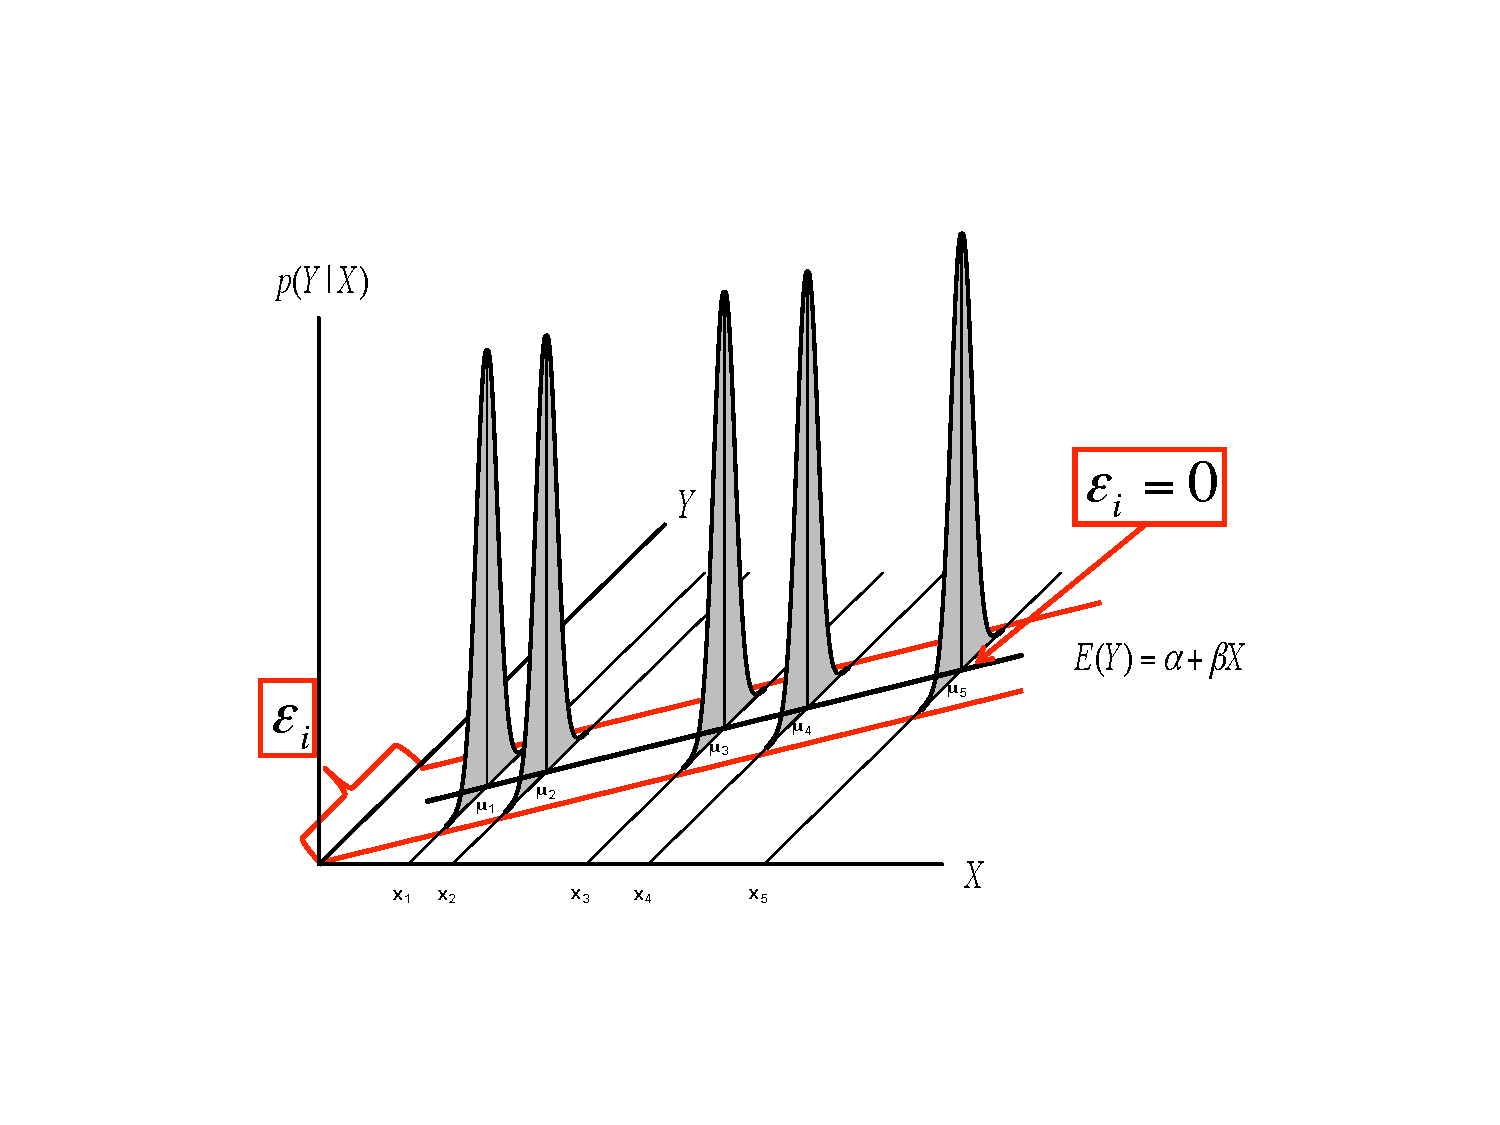
\includegraphics[width=4in]{../10_SimpleDiagnostics/residdist.pdf}%filename
  \caption{Assumed Distributions of OLS Residuals \label{fig:residdist}}
\end{figure}

How can we determine whether our residuals approximate the expected pattern? The most straight-forward approach is to visually examine the distribution of the residuals over the range of the predicted values for $Y$. If all is well, there should be no obvious pattern to the residuals -- they should appear as a ``sneeze plot" (i.e.,  it looks like you sneezed on the plot. How gross!) as shown in Figure \ref{fig:sneeze}.

\begin{figure}
  \centering
  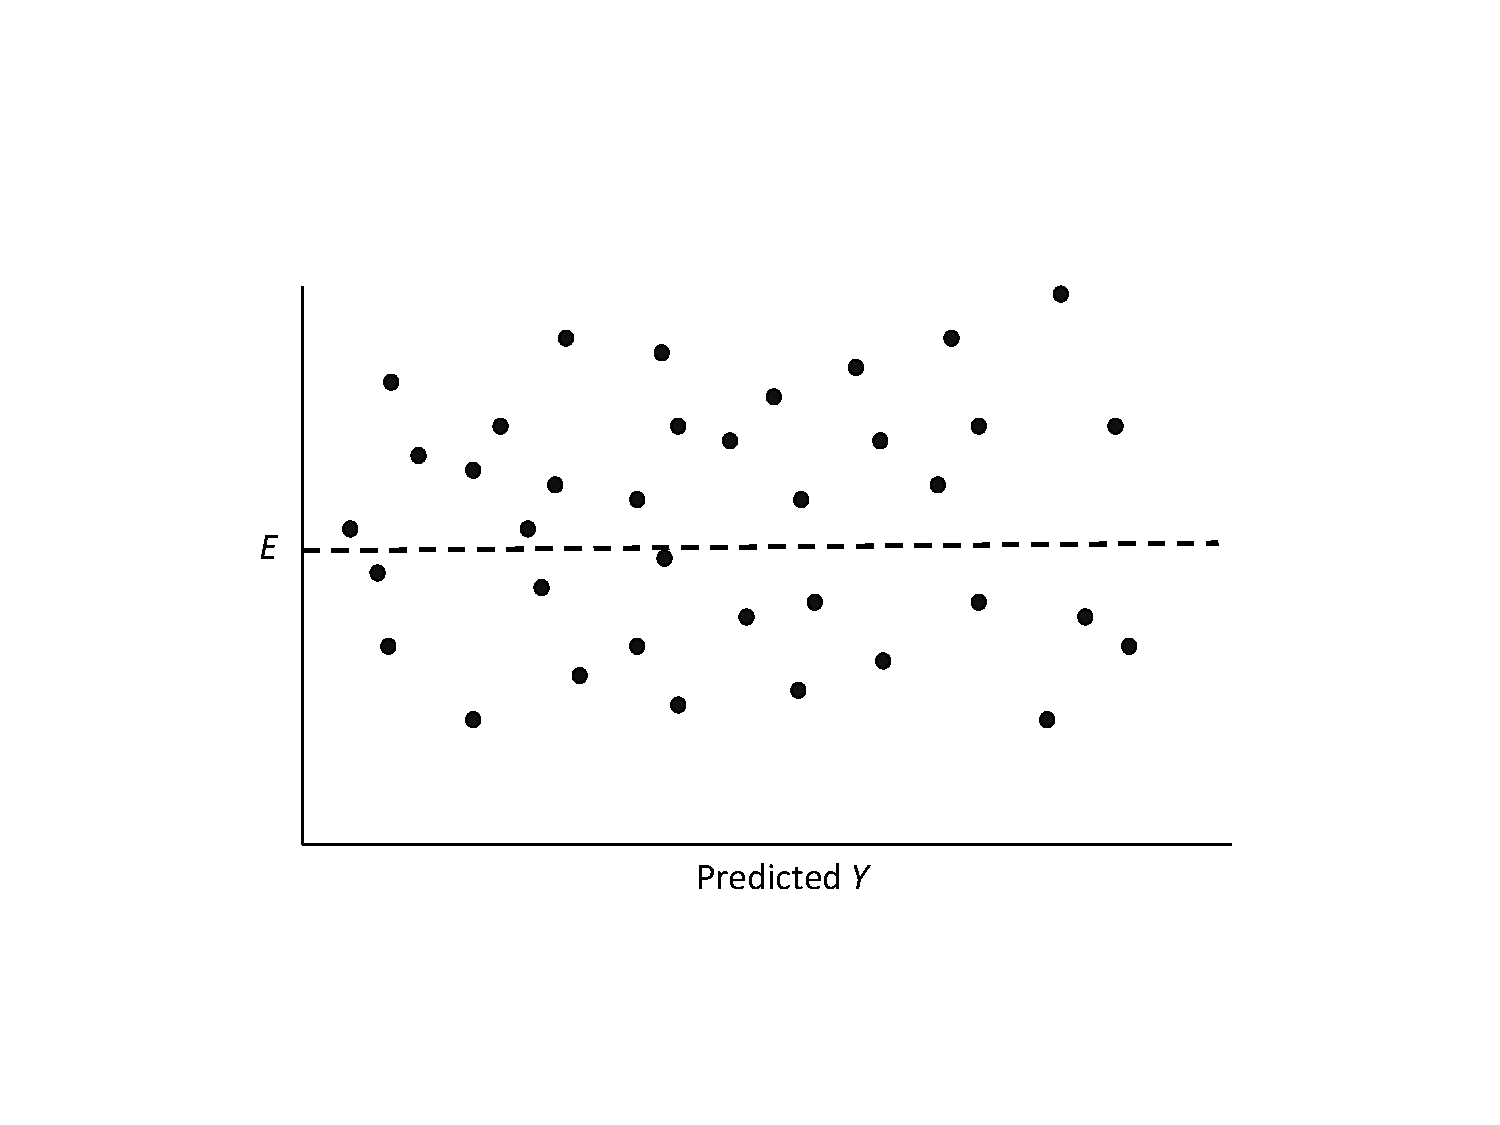
\includegraphics[width=4in]{../10_SimpleDiagnostics/sneeze.pdf}%filename
  \caption{Ideal Pattern of Residuals from a Simple OLS Model \label{fig:sneeze}}
\end{figure}

Generally, there is no pattern in such a sneeze plot of residuals. One of the difficulties we have, as human beings, is that we tend to look at randomness and \texttt{perceive} patterns. Our brains are wired to see patterns, even where their are none. Moreover, with random distributions there will in some samples be clumps and gaps that do \texttt{appear} to depict some kind of order when in fact there is none. There is the danger, then, of over-interpreting the pattern of residuals to see problems that aren't there. The key is to know what kinds of patterns to look for, so when you do observe one you will know it.

\section{When Things Go Bad with Residuals} 

Residual analysis is the process of looking for \texttt{signature patterns} in the residuals that are indicative of failure in the underlying assumptions of OLS regression. Different kinds of problems lead to different patterns in the residuals.

\subsection{``Outlier" Data}

Sometimes our data include unusual cases that behave differently from most of our observations. This may happen for a number of reasons. The most typical is that the data have been mis-coded, with some subgroup of the data having numerical values that lead to large residuals. Cases like this can also arise when a subgroup of the cases differ from the others in how $X$ influences $Y$, and that difference has not been captured in the model. This is a problem referred to as the omission of important independent variables.\footnote{Political scientists who study US electoral politics have had to account for unusual observations in the Southern states. Failure in the model to account for these differences would lead to prediction error and ugly patterns in the residuals. Sadly, Professor Gaddie notes that scholars have not been sufficiently careful -- or perhaps well-trained? -- to do this right. Professor Gaddie notes:  ``... instead of working to achieve better model specification through the application of theory and careful thought, in the 1960s and 1970s electoral scholars instead just threw out the South and all senate races, creating the perception that the United States had 39 states and a unicameral legislature."} Figure \ref{fig:unusual_dat} shows a stylized example, with a cluster of residuals falling at considerable distance from the rest. 

\begin{figure}
  \centering
  \includegraphics[width=4in]%
    {../10_SimpleDiagnostics/unusual_dat.pdf}% picture filename
  \caption{Unusual Data Patterns in Residuals \label{fig:unusual_dat}}
\end{figure}

This is a case of influential outliers. The effect of such outliers can be significant, as the OLS estimates of $A$ and $B$ seek to minimize overall squared error. In the case of Figure \ref{fig:unusual_dat}, the effect would be to shift the estimate of $B$ to accommodate the unusual observations, as illustrated in Figure \ref{fig:unusual_dat2}. One possible response would be to omit the unusual observations, as shown in Figure \ref{fig:unusual_dat2}. Another would be to consider, theoretically and empirically, why these observations are unusual. Are they, perhaps, miscoded? Or are they codes representing missing values (e.g., ``-99")?

If they are not mis-codes, perhaps these outlier observations manifest a different kind of relationship between $X$ and $Y$, which might in turn require a revised theory and model. We will address some modeling options to address this possibility when we explore multiple regression, in Part III of this book.

\begin{figure}
  \centering
  \includegraphics[width=4in]%
    {../10_SimpleDiagnostics/unusual_dat2.pdf}% picture filename
  \caption{Implications of Unusual Data Patterns in Residuals \label{fig:unusual_dat2}}
\end{figure}

In sum, outlier analysis looks at residuals for patterns in which some observations deviate widely from others. If that deviation is influential, changing estimates of $A$ and $B$ as shown in Figure \ref{fig:unusual_dat2}, then you must examine the observations to determine whether they are mis-coded. If not, you can evaluate whether the cases are theoretically distinct, such that the influence of $X$ on $Y$ is likely to be different than for other cases. If you conclude that this is so, you will need to respecify your model to account for these differences. We will discuss some options for doing that later in this chapter, and again in our discussion of multiple regression.

\subsection{Non-Constant Variance}

A second thing to look for in visual diagnostics of residuals is non-constant variance, or
\texttt{heteroscedasticity}. In this case, the variation in the residuals over the range of predicted values for $Y$ should be roughly even. A problem occurs when that variation changes substantially as the predicted value of $Y$ changes, as is illustrated in Figure \ref{fig:hetero10}.

\begin{figure}
  \centering
  \includegraphics[width=4in]%
    {../10_SimpleDiagnostics/hetero.pdf}% picture filename
  \caption{Non-Constant Variance in the Residuals \label{fig:hetero10}}
\end{figure}

As Figure \ref{fig:hetero10} shows, the width of the spread of the residuals grows as the predicted value of $Y$ increases, making a fan-shaped pattern. Equally concerning would be a case of a ``reverse fan", or a pattern with a bulge in the middle and very ``tight" distributions of residuals at either extreme. These would all be cases in which the assumption of constant-variance in the residuals (or ``homoscedasticity") fails, and are referred to as instances of heteroscedasticity.

What are the implications of heteroscedasticity? Our hypothesis tests for the estimated coefficients ($A$ and $B$) are based on the assumption that the standard errors of the estimates (see the prior chapter) are normally distributed. If inspection of your residuals provides evidence to question that assumption, then the interpretation of the t-values and p-values may be problematic. Intuitively, in such a case the precision of our estimates of $A$ and $B$ are not constant -- but rather will depend on the predicted value of $Y$. So you might be estimating $B$ relatively precisely in some ranges of $Y$, and less precisely in others. That means you cannot depend on the estimated t and p-values to test your hypotheses.

\subsection{Non-Linearity in the Parameters}

One of the primary assumptions of simple OLS regression is that the estimated slope parameter (the $B$) will be constant, and therefore the model will be linear. Put differently, the effect of any change in $X$ on $Y$  should be constant over the range of $Y$. Thus, if our assumption is correct, the pattern of the residuals should be roughly symmetric, above and below zero, over the range of predicted values.

If the real relationship between $X$ and $Y$ is not linear, however, the predicted (linear) values for $Y$ will systematically depart from the (curved) relationship that is represented in the data. Figure \ref{fig:simplenonlin} shows the kind of pattern we would expect in our residuals if the observed relationship between $X$ and $Y$ is a strong curve, when we attempt to model it as if it were linear.

\begin{figure}
  \centering
  \includegraphics[width=4in]%
    {../10_SimpleDiagnostics/simplenonlin.pdf}% picture filename
  \caption{Non-Linearity in the Residuals \label{fig:simplenonlin}}
\end{figure}

What are the implications of non-linearity? First, because the slope is non-constant, the estimate of $B$ will be biased. In the illustration shown in Figure \ref{fig:simplenonlin}, $B$ would underestimate the value of $Y$ in both the low and high ranges of the predicted value of $Y$, and overestimate it in the mid-range. In addition, the standard errors of the residuals will be large, due to systematic over- and under-estimation of $Y$, making the model very inefficient (or imprecise). 

\section{Application of Residual Diagnostics}

This far we have used rather simple illustrations of residual diagnostics and the kinds of patterns to look for. But you should be warned that, in real applications, the patterns are rarely so clear. So we will walk through an example diagnostic session, using the the \texttt{tbur} data set.

Our in-class lab example focuses on the relationship between political ideology (``ideology" in our dataset) as a predictor of the perceived risks posed by climate change (``gccrsk"). The model is specified in \texttt{R} as follows:

\begin{knitrout}
\definecolor{shadecolor}{rgb}{0.969, 0.969, 0.969}\color{fgcolor}\begin{kframe}
\begin{alltt}
\hlstd{OLS_env} \hlkwb{<-} \hlkwd{lm}\hlstd{(ds}\hlopt{$}\hlstd{glbcc_risk} \hlopt{~} \hlstd{ds}\hlopt{$}\hlstd{ideol)}
\end{alltt}
\end{kframe}
\end{knitrout}

\noindent Using the summary command in $R$, we can review the results.
\begin{knitrout}
\definecolor{shadecolor}{rgb}{0.969, 0.969, 0.969}\color{fgcolor}\begin{kframe}
\begin{alltt}
\hlkwd{summary}\hlstd{(OLS_env)}
\end{alltt}
\begin{verbatim}
## 
## Call:
## lm(formula = ds$glbcc_risk ~ ds$ideol)
## 
## Residuals:
##    Min     1Q Median     3Q    Max 
## -8.726 -1.633  0.274  1.459  6.506 
## 
## Coefficients:
##             Estimate Std. Error t value Pr(>|t|)    
## (Intercept) 10.81866    0.14189   76.25   <2e-16 ***
## ds$ideol    -1.04635    0.02856  -36.63   <2e-16 ***
## ---
## Signif. codes:  0 '***' 0.001 '**' 0.01 '*' 0.05 '.' 0.1 ' ' 1
## 
## Residual standard error: 2.479 on 2511 degrees of freedom
##   (34 observations deleted due to missingness)
## Multiple R-squared:  0.3483,	Adjusted R-squared:  0.348 
## F-statistic:  1342 on 1 and 2511 DF,  p-value: < 2.2e-16
\end{verbatim}
\end{kframe}
\end{knitrout}

Note that, as was discussed in the prior chapter, the estimated value for $B$ is negative and highly statistically significant. This indicates that the more conservative the survey respondent, the lower the perceived risks attributed to climate change. Now we will use these model results and the associated residuals to evaluate the key assumptions of OLS, beginning with linearity. 

\subsection{Testing for Non-Linearity}
One way to test for non-linearity is to fit the model to a polynomial functional form. This sounds impressive, but is quite easy to do and understand (really!). All you need to do is include the square of the independent variable as a second predictor in the model.  A significant regression coefficient on the squared variable indicates problems with linearity. To do this, we first produce the squared variable.

\begin{knitrout}
\definecolor{shadecolor}{rgb}{0.969, 0.969, 0.969}\color{fgcolor}\begin{kframe}
\begin{alltt}
\hlcom{#first we square the ideology variable and create a new variable to use in our model.}
\hlstd{ds}\hlopt{$}\hlstd{ideology2} \hlkwb{<-} \hlstd{ds}\hlopt{$}\hlstd{ideol}\hlopt{^}\hlnum{2}
\hlkwd{summary}\hlstd{(ds}\hlopt{$}\hlstd{ideology2)}
\end{alltt}
\begin{verbatim}
##    Min. 1st Qu.  Median    Mean 3rd Qu.    Max.    NA's 
##    1.00   16.00   25.00   24.65   36.00   49.00      23
\end{verbatim}
\end{kframe}
\end{knitrout}

\noindent Next, we run the regression with the original independent variable and our new squared variable.  Finally, we check the regression output.

\begin{knitrout}
\definecolor{shadecolor}{rgb}{0.969, 0.969, 0.969}\color{fgcolor}\begin{kframe}
\begin{alltt}
\hlstd{OLS_env2} \hlkwb{<-} \hlkwd{lm}\hlstd{(glbcc_risk} \hlopt{~} \hlstd{ideol} \hlopt{+} \hlstd{ideology2,} \hlkwc{data} \hlstd{= ds)}
\hlkwd{summary}\hlstd{(OLS_env2)}
\end{alltt}
\begin{verbatim}
## 
## Call:
## lm(formula = glbcc_risk ~ ideol + ideology2, data = ds)
## 
## Residuals:
##    Min     1Q Median     3Q    Max 
## -8.564 -1.808  0.192  1.448  6.863 
## 
## Coefficients:
##             Estimate Std. Error t value Pr(>|t|)    
## (Intercept)  9.58238    0.28397  33.745  < 2e-16 ***
## ideol       -0.34444    0.14274  -2.413   0.0159 *  
## ideology2   -0.08234    0.01641  -5.018 5.58e-07 ***
## ---
## Signif. codes:  0 '***' 0.001 '**' 0.01 '*' 0.05 '.' 0.1 ' ' 1
## 
## Residual standard error: 2.467 on 2510 degrees of freedom
##   (34 observations deleted due to missingness)
## Multiple R-squared:  0.3548,	Adjusted R-squared:  0.3543 
## F-statistic: 690.1 on 2 and 2510 DF,  p-value: < 2.2e-16
\end{verbatim}
\end{kframe}
\end{knitrout}
A significant coefficient on the squared ideology variable informs us that we probably have a non-linearity problem. The significant and negative coefficient for the square of ideology means that the curve steepens (perceived risks fall faster) as the scale shifts further up on the conservative side of the scale. We can supplement the polynomial regression test by producing a residual plot with a formal Tukey test. The residual plot (\texttt{car} package \texttt{residualPlots} function) displays the Pearson fitted values against the model's observed values. Ideally, the plots will produce flat red lines; curved lines represent non-linearity.  The output for the Tukey test is visible in the $R$ workspace.  The null hypothesis for the Tukey test is a linear relationship, so a significant p-value is indicative of non-linearity.  The tukey test is reported as part of the \texttt{residualPlots} function in the \texttt{car} package.

\begin{knitrout}
\definecolor{shadecolor}{rgb}{0.969, 0.969, 0.969}\color{fgcolor}\begin{kframe}
\begin{alltt}
\hlcom{#A significant p-value indicates non-linearity using the Tukey test}
\hlkwd{residualPlots}\hlstd{(OLS_env)}
\end{alltt}
\begin{verbatim}
##            Test stat Pr(>|Test stat|)    
## ds$ideol     -5.0181        5.584e-07 ***
## Tukey test   -5.0181        5.219e-07 ***
## ---
## Signif. codes:  0 '***' 0.001 '**' 0.01 '*' 0.05 '.' 0.1 ' ' 1
## pdf 
##   2
\end{verbatim}
\end{kframe}
\end{knitrout}

\begin{figure}
  \centering
  \includegraphics[width=4in]%
    {../10_SimpleDiagnostics/nonlinideology.pdf}% picture filename
  \caption{Residual Plots Examining Model Linearity \label{fig:nonlinideology}}
\end{figure}

The curved red lines in Figure \ref{fig:nonlinideology} in the residual plots and significant Tukey test indicate a non-linear relationship in the model.  This is a serious violation of a core assumption of OLS regression, which means that the estimate of $B$ is likely to be biased. Our findings suggest that the relationship between ideology and perceived risks of climate change is approximately linear from ``strong liberals" to those who are ``leaning Republican". But perceived risks seem to drop off more rapidly as the scale rises toward ``strong Republican."

\subsection{Testing for Normality in Model Residuals}
Testing for normality in the model residuals will involve using many of the techniques demonstrated in previous chapters.  The first step is to  graphically display the residuals in order to see how closely the model residuals resemble a normal distribution.  A formal test for normality is also included in the demonstration.

Start by creating a histogram of the model residuals.

\begin{knitrout}
\definecolor{shadecolor}{rgb}{0.969, 0.969, 0.969}\color{fgcolor}\begin{kframe}
\begin{alltt}
\hlstd{OLS_env}\hlopt{$}\hlstd{residuals} \hlopt \hlcom{# Pipe the residuals to a data frame}
  \hlkwd{data.frame}\hlstd{()} \hlopt \hlcom{# Pipe the data frame to ggplot}
  \hlkwd{ggplot}\hlstd{(}\hlkwd{aes}\hlstd{(OLS_env}\hlopt{$}\hlstd{residuals))} \hlopt{+}
  \hlkwd{geom_histogram}\hlstd{(}\hlkwc{bins} \hlstd{=} \hlnum{16}\hlstd{)}
\end{alltt}
\end{kframe}
\end{knitrout}

\begin{figure}
  \centering
  \includegraphics[width=4in]%
    {../10_SimpleDiagnostics/histideology.pdf}% picture filename
  \caption{Histogram of Model Residuals \label{fig:histideology}}
\end{figure}

The histogram in figure \ref{fig:histideology} indicates that the residuals are approximately normally distributed, but there appears to be a negative skew.  Next, we can create a smoothed density of the model residuals compared to a theoretical normal distribution.

\begin{knitrout}
\definecolor{shadecolor}{rgb}{0.969, 0.969, 0.969}\color{fgcolor}\begin{kframe}
\begin{alltt}
\hlstd{OLS_env}\hlopt{$}\hlstd{residuals} \hlopt \hlcom{# Pipe the residuals to a data frame}
  \hlkwd{data.frame}\hlstd{()} \hlopt \hlcom{# Pipe the data frame to ggplot}
  \hlkwd{ggplot}\hlstd{(}\hlkwd{aes}\hlstd{(OLS_env}\hlopt{$}\hlstd{residuals))} \hlopt{+}
  \hlkwd{geom_density}\hlstd{(}\hlkwc{adjust} \hlstd{=} \hlnum{2}\hlstd{)} \hlopt{+}
  \hlkwd{stat_function}\hlstd{(}\hlkwc{fun} \hlstd{= dnorm,} \hlkwc{args} \hlstd{=} \hlkwd{list}\hlstd{(}\hlkwc{mean} \hlstd{=} \hlkwd{mean}\hlstd{(OLS_env}\hlopt{$}\hlstd{residuals),}
                                         \hlkwc{sd} \hlstd{=} \hlkwd{sd}\hlstd{(OLS_env}\hlopt{$}\hlstd{residuals)),}
                \hlkwc{color} \hlstd{=} \hlstr{"red"}\hlstd{)}
\hlkwd{dev.off}\hlstd{()}
\end{alltt}
\end{kframe}
\end{knitrout}

\begin{figure}
  \centering
  \includegraphics[width=4in]%
    {../10_SimpleDiagnostics/densityideology.pdf}% picture filename
  \caption{Smoothed Density Plot of Model Residuals \label{fig:densityideology}}
\end{figure}
\FloatBarrier

Figure \ref{fig:densityideology} indicates the model residuals deviate slightly from a normal distributed because of a slightly negative skew and a mean higher than we would expect in a normal distribution.  Our final ocular examination of the residuals will be a quartile plot (using the \texttt{stat_qq} function from the \texttt{ggplot2} package).

\begin{knitrout}
\definecolor{shadecolor}{rgb}{0.969, 0.969, 0.969}\color{fgcolor}\begin{kframe}
\begin{alltt}
\hlstd{OLS_env}\hlopt{$}\hlstd{residuals} \hlopt \hlcom{# Pipe the residuals to a data frame}
  \hlkwd{data.frame}\hlstd{()} \hlopt \hlcom{# Pipe the data frame to ggplot}
  \hlkwd{ggplot}\hlstd{(}\hlkwd{aes}\hlstd{(}\hlkwc{sample} \hlstd{= OLS_env}\hlopt{$}\hlstd{residuals))} \hlopt{+}
  \hlkwd{stat_qq}\hlstd{()} \hlopt{+}
  \hlkwd{stat_qq_line}\hlstd{()}
\hlkwd{dev.off}\hlstd{()}
\end{alltt}
\end{kframe}
\end{knitrout}


\begin{figure}
  \centering
  \includegraphics[width=4in]%
    {../10_SimpleDiagnostics/QQideology.pdf}% picture filename
  \caption{Quartile Plot of Model Residuals \label{fig:QQideology}}
\end{figure}
\FloatBarrier

According to Figure \ref{fig:QQideology}, it appears as if the residuals are normally distributed except for the tails of the distribution.   Taken together the graphical representations of the residuals suggest modest non-normality.  As a final step, we can conduct a formal Shapiro-Wilk test for normality.  The null hypothesis for a Shapiro-Wilk test is a normal distribution, so we do not want to see a significant p-value.

\begin{knitrout}
\definecolor{shadecolor}{rgb}{0.969, 0.969, 0.969}\color{fgcolor}\begin{kframe}
\begin{alltt}
\hlcom{#a significant value p-value potentially indicates the data is not normally distributed.}
\hlkwd{shapiro.test}\hlstd{(OLS_env}\hlopt{$}\hlstd{residuals)}
\end{alltt}
\begin{verbatim}
## 
## 	Shapiro-Wilk normality test
## 
## data:  OLS_env$residuals
## W = 0.98901, p-value = 5.51e-13
\end{verbatim}
\end{kframe}
\end{knitrout}

The Shapiro-Wilk test confirms what we observed in the graphical displays of the model residuals -- the residuals are not normally distributed.   Recall that our dependent variable (gccrsk) appears to have a non-normal distribution. This could be the root of the non-normality found in  the model residuals. Given this information, steps must be taken to assure that the model residuals meet the required OLS assumptions. One possibility would be to transform the dependent variable (glbccrisk) in order to induce a normal distribution. Another might be to add a polynomial term to the independent variable (ideology) as was done above. In either case, you would need to recheck the residuals in order to see if the model revisions adequately dealt with the problem. We suggest that you do just that!

\subsection{Testing for Non-Constant Variance in the Residuals}

Testing for non-constant variance (heteroscedasticity) in a model is fairly straightforward. We can start by creating a spread-level plot  that fits the studentized residuals against the model's fitted values.  A line with a non-zero slope is indicative of heteroscedasticity. Figure \ref{fig:spreadlvlideology} displays the spread-level plot from the \texttt{car} package.

\begin{knitrout}
\definecolor{shadecolor}{rgb}{0.969, 0.969, 0.969}\color{fgcolor}\begin{kframe}
\begin{alltt}
\hlkwd{spreadLevelPlot}\hlstd{(OLS_env)}
\end{alltt}
\end{kframe}
\end{knitrout}

\begin{figure}
  \centering
  \includegraphics[width=4in]%
    {../10_SimpleDiagnostics/spreadlvlideology.pdf}% picture filename
  \caption{Spread-Level Plot of Model Residuals \label{fig:spreadlvlideology}}
\end{figure}
\FloatBarrier

The negative slope on the red line in Figure \ref{fig:spreadlvlideology} indicates the model may contain heteroscedasticity.  We can also perform  a formal test for non constant variance.  The null hypothesis is constant variance, so we do not want to see a significant p-value.

\begin{knitrout}
\definecolor{shadecolor}{rgb}{0.969, 0.969, 0.969}\color{fgcolor}\begin{kframe}
\begin{alltt}
\hlcom{#a significant value indicates potential heteroscedasticity issues.}
\hlkwd{ncvTest}\hlstd{(OLS_env)}
\end{alltt}
\begin{verbatim}
## Non-constant Variance Score Test 
## Variance formula: ~ fitted.values 
## Chisquare = 68.107    Df = 1     p = 1.548597e-16
\end{verbatim}
\end{kframe}
\end{knitrout}

The significant p-value on the non-constant variance test informs us that there is a problem with heteroscedasticity in the model.  This is yet another violation of the core assumptions of OLS regression, and it brings into doubt our hypothesis tests.

\subsection{Examining Outlier Data}

There are a number of ways to examine outlying observations in an OLS regression. This section briefly illustrates a a subset of analytical tests that will provide a useful assessment of potentially important outliers.  The purpose of examining outlier data is twofold.  First, we want to make sure there are not any mis-coded or invalid data influencing our regression. For example, an outlying observation with a value of ``-99" would very likely bias our results, and obviously needs to be  corrected. Second, outlier data may indicate the need to theoretically reconceptualize our model.  Perhaps the relationship in the model is mis-specified, with outliers at the extremes of a variable suggesting a non-linear relationship. Or it may be that a  subset of cases respond differently to the independent variable, and therefore must be treated as ``special cases" in the model. Examining outliers allows us to identify and address these potential problems.

One of the first things we can do is perform a Bonferroni Outlier Test. The Bonferroni Outlier Tests uses a $t$ distribution to test whether the model's largest studentized residual value's outlier status is statistically different from the other observations in the model.  A significant p-value indicates an extreme outlier that warrants further examination.  We use the \texttt{outlierTest} function in the \texttt{car} package to perform a Bonferroni Outlier Test.

\begin{knitrout}
\definecolor{shadecolor}{rgb}{0.969, 0.969, 0.969}\color{fgcolor}\begin{kframe}
\begin{alltt}
\hlcom{#a significant p-value indicates extreme case for review}
\hlkwd{outlierTest}\hlstd{(OLS_env)}
\end{alltt}
\begin{verbatim}
## No Studentized residuals with Bonferonni p < 0.05
## Largest |rstudent|:
##      rstudent unadjusted p-value Bonferonni p
## 589 -3.530306         0.00042255           NA
\end{verbatim}
\end{kframe}
\end{knitrout}

According to the R output, the Bonferroni p-value for the largest (absolute) residual is not statistically significant.  While this test is important for identifying a potentially significant outlying  observation, it is not a panacea for checking for patterns in outlying data.  Next we will examine the model's df.betas in order to see which observations exert the most influence on the model's regression coefficients. $Dfbetas$ are measures of how much the regression coefficient changes when observation $i$ is omitted.  Larger values indicate an observation that has considerable influence on the model.   

A useful method for finding dfbeta obervations is to use the \texttt{dfbetaPlots} function in the \texttt{car} package.  We specify the option \texttt{id.n=2} to show the two largest df.betas.  See figure \ref{fig:dfbetaPlots}.

\begin{knitrout}
\definecolor{shadecolor}{rgb}{0.969, 0.969, 0.969}\color{fgcolor}\begin{kframe}
\begin{alltt}
\hlstd{plotdb}\hlkwb{<-}\hlkwd{dfbetaPlots}\hlstd{(OLS_env,} \hlkwc{id.n}\hlstd{=}\hlnum{3}\hlstd{)}
\end{alltt}
\end{kframe}
\end{knitrout}

\begin{figure}
  \centering
  \includegraphics[width=4in]%
    {../10_SimpleDiagnostics/dfbetaPlots.pdf}% picture filename
  \caption{Plot of Model dfbetas Values using \texttt{dfbetaPlots} function \label{fig:dfbetaPlots}}
\end{figure}
\FloatBarrier

\begin{knitrout}
\definecolor{shadecolor}{rgb}{0.969, 0.969, 0.969}\color{fgcolor}\begin{kframe}
\begin{alltt}
\hlcom{#  Check the observations with high dfbetas.}
\hlcom{#  We see the values 589 and 615 returned.  }
\hlcom{#  We only want to see results from columns gccrsk and ideology in tbur.data.}
\hlstd{ds[}\hlkwd{c}\hlstd{(}\hlnum{589}\hlstd{,}\hlnum{615}\hlstd{),}\hlkwd{c}\hlstd{(}\hlstr{"glbcc_risk"}\hlstd{,} \hlstr{"ideol"}\hlstd{)]}
\end{alltt}
\begin{verbatim}
##     glbcc_risk ideol
## 589          0     2
## 615          0     2
\end{verbatim}
\end{kframe}
\end{knitrout}

These observations are interesting because they identify a potential problem in our model specification.  Both observations are considered outliers because the respondents self-identified as ``liberal" (ideology = 1) and rated their perceived  risk of global climate change as 0.  These values deviate substantially from the norm for other strong liberals in the dataset.  Remember, as we saw earlier, our model has a problem with non-linearity -- these outlying observations seem to corroborate this finding.  Examination of outliers sheds some light on the issue.

Finally, we can produce a plot that combines studentized residuals, ``hat values", and Cook's D distances (these are measures of the amount of influence observations have on the model) using circles as an indicator of influence -- the larger the circle, the greater the influence.  Figure \ref{fig:bubbleideology2} displays the combined influence plot.  In addition, the \texttt{influencePlot} function returns the values of greatest influence.

\begin{knitrout}
\definecolor{shadecolor}{rgb}{0.969, 0.969, 0.969}\color{fgcolor}\begin{kframe}
\begin{alltt}
\hlkwd{influencePlot}\hlstd{(OLS_env)}
\end{alltt}
\begin{verbatim}
##         StudRes         Hat        CookD
## 20   0.09192603 0.002172497 9.202846e-06
## 30   0.09192603 0.002172497 9.202846e-06
## 589 -3.53030574 0.001334528 8.289419e-03
## 615 -3.53030574 0.001334528 8.289419e-03
## pdf 
##   2
\end{verbatim}
\end{kframe}
\end{knitrout}

\begin{figure}
  \centering
  \includegraphics[width=4in]%
    {../10_SimpleDiagnostics/bubbleideology.pdf}% picture filename
  \caption{Influence Bubble Plot \label{fig:bubbleideology2}}
\end{figure}
\FloatBarrier

\noindent Figure \ref{fig:bubbleideology2} indicates that there are a number of cases that warrant further examination.  We are already familiar with 589 and 615  Let's add 20, 30, 90 and 1052.

\begin{knitrout}
\definecolor{shadecolor}{rgb}{0.969, 0.969, 0.969}\color{fgcolor}\begin{kframe}
\begin{alltt}
\hlcom{#review the results}
\hlstd{ds[}\hlkwd{c}\hlstd{(}\hlnum{589}\hlstd{,}\hlnum{615}\hlstd{,}\hlnum{20}\hlstd{,}\hlnum{30}\hlstd{,}\hlnum{90}\hlstd{,}\hlnum{1052}\hlstd{),}\hlkwd{c}\hlstd{(}\hlstr{"glbcc_risk"}\hlstd{,} \hlstr{"ideol"}\hlstd{)]}
\end{alltt}
\begin{verbatim}
##      glbcc_risk ideol
## 589           0     2
## 615           0     2
## 20           10     1
## 30           10     1
## 90           10     1
## 1052          3     6
\end{verbatim}
\end{kframe}
\end{knitrout}

One important take-away from a visual examination of these observations is that there do not appear to be any completely mis-coded or invalid data affecting our model. In general, even the most influential observations do not appear to be implausible cases.  Observations 589 and 615 \footnote{Of note, observations 20, 30, and 90 and 1052 are returned as well.  There doesn't appear to be anything special about these four observations.  Part of this may be due to the bivariate relationship and how the \texttt{influcencePlot} function weights the data.  The results are included for your review.} present an interesting problem regarding  theoretical and model specification. These observations represent respondents who self-reported as  ``liberal" (ideology=2) and also rated the perceived risk of global climate change as 0 out of 10. These observations therefore deviate from the model's expected values (``strong liberal" respondents, on average, believed global climate change represents a high risk).  Earlier in our diagnostic testing we found a problem with non-linearity. Taken together, it looks like the non-linearity in our model is due to observations at the ideological extremes.  One way we can deal with this problem is to include a squared ideology variable (a polynomial) in the model, as illustrated earlier in this chapter. However, it is also important to note this non-linear relationship in the theoretical conceptualization of our model. Perhaps there is something special about people with extreme ideologies that needs to be taken into account when attempting to predict perceived risk of global climate change. This finding should also inform our examination of post-estimation predictions -- something that will be covered later in this text.

\section{So Now What? Implications of Residual Analysis}

What should you do if you observe patterns in the residuals that seem to violate the assumptions of OLS? If you find deviant cases -- outliers that are shown to be highly influential -- you need to first evaluate the specific cases (observations). Is it possible that the data were miscoded? We hear of many instances in which missing value codes (often ``-99") were inadvertently left in the dataset. \texttt{R} would treat such values as if they were real data, often generating glaring and influential outliers. Should that be the case, recode the offending variable observation as missing (``NA") and try again.  

%for future reference - http://connectmv.com/tutorials/r-tutorial/investigating-outliers-discrepancies-and-other-influential-points/
% we can use a process to quickly remove the results.

But what if there is no obvious coding problem? It may be that the influential outlier is appropriately measured, but that the observation is different in some theoretically important way. Suppose, for example, that your model included some respondents who -- rather than diligently answering your questions -- just responded at random to your survey questions. They would introduce noise and error. If you could measure these slackers, you could either exclude them or include a control variable in your model to account for their different patterns of responses. We will discuss inclusion of model controls when we turn to multiple regression modeling in later chapters.

What if your residual analysis indicates the presence of heteroscedasticity? Recall that this will undermine your ability to do hypothesis tests in OLS. There are several options. If the variation in fit over the range of the predicted value of $Y$ could plausibly result from the omission of an important explanatory variable, you should respecify your model accordingly (more on this later in this book). It is often the case that you can improve the distribution of residuals by including important but previously omitted variables. Measures of income, when left out of consumer behavior models, often have this effect.

Another approach is to use a different modeling approach that accounts for the heteroscedasticity in the estimated standard error. Of particular utility are robust estimators, which can be employed using the \texttt{rlm} (robust linear model) function in the \texttt{MASS} package. This approach increases the magnitude of the estimated standard errors, reducing the t-values and resulting p-values. That means that the ``cost" of running robust estimators is that the precision of the estimates is reduced.

Evidence of non-linearity in the residuals presents a thorny problem. This is a basic violation of a central assumption of OLS, resulting in biased estimates of $A$ and $B$. What can you do? First, you can respecify your model to include a polynomial; you would include both the $X$ variable and a square of the $X$ variable. Note that this will require you to recode $X$. In this approach, the value of $X$ is constant, while the value of the square of $X$ increases exponentially. So a relationship in which $Y$ decreases as the square of $X$ increases will provide a progressively steeper slope as $X$ rises. This is the kind of pattern we observed in the example in which political ideology was used to predict the perceived risk posed by climate change.

\section{Summary} 

Now you are in a position to employ diagnostics -- both visual and statistical -- to evaluate the results of your statistical models. Note that, once you have made your model corrections, you will need to regenerate and re-evaluate your model residuals to determine whether the problem has been ameliorated. Think of diagnostics as an iterative process in which you use the model results to evaluate, diagnose, revise re-run, and re-evaluate your model. This is where the real learning happens, as you challenge your theory (as specified in your model) with observed data. So -- have at it!
\end{document}
